\chapter{Introducción específica} % Main chapter title
\label{Chapter2}

%----------------------------------------------------------------------------------------
%	SECTION 1
%----------------------------------------------------------------------------------------
En este capítulo se presentan una introducción al trabajo realizado así como los requerimientos del sistema que fueron oportunamente consensuados con el cliente. Posteriormente, se realiza una descripción de las tecnologías utilizadas.

\section{Estructura general del sistema}

En la figura \ref{fig:diagBloques} se muestra el diagrama en bloques simplificado del sistema. En la figura se observa el dispositivo diseñado, el cual se encuentra dentro de un recuadro, y el transformador a ensayar. Dentro del dispositivo diseñado se observan los siguientes bloques principales:

\begin{itemize}
\item Módulo ESP32 con Wi-Fi integrado.
\item Bloques de acondicionamiento de señal y actuación para el bobinado primario y secundario.
\item Interfaz de usuario: pulsadores, \textit{display} y \textit{buzzer}.
\item Interfaz serie para impresora.
\item \textit{Switch} de seguridad. Se utiliza para indicar que la tapa de seguridad ha sido removida y el operario puede quedar expuesto a altas tensiones.
\item Fuente de alimentación.
\end{itemize}

El trabajo desarrollado tiene como fin determinar si un transformador dado es apto o no para ser utilizado en determinados equipos. Para tal fin, se configuran umbrales de comparación por medio de una comunicación HTTP a un servidor web y se procede a compararlos contra mediciones realizadas sobre el transformador. Una vez realizadas las comparaciones, los resultados del ensayo se muestran localmente por medio de un \textit{display}. Adicionalmente, los resultados y las mediciones realizadas son enviadas al servidor web del cliente utilizando el protocolo HTTP. Por otro lado, se cuenta con una impresora la cual imprime una etiqueta que permite la trazabilidad del transformador.

Todo el dispositivo es controlado por solo tres pulsadores: Testear, Configurar y Cancelar.

A continuación se detalla un resumen de las tareas realizadas en este trabajo:
\begin{itemize}
\item Mediciones de tensión y corriente a los transformadores bajo ensayo.
\item Pedido de umbrales de aceptación a un servidor web.
\item Emisión de aceptación o rechazo del transformador.
\item Visualización en el \textit{display} de los umbrales configurados y las mediciones realizadas.
\item Envío de las mediciones a un servidor web por medio del protocolo HTTP.
\item Gestión de la conexión Wi-Fi.
\item Impresión de etiquetas. 
\end{itemize}

\begin{figure}[htpb]
\centering 
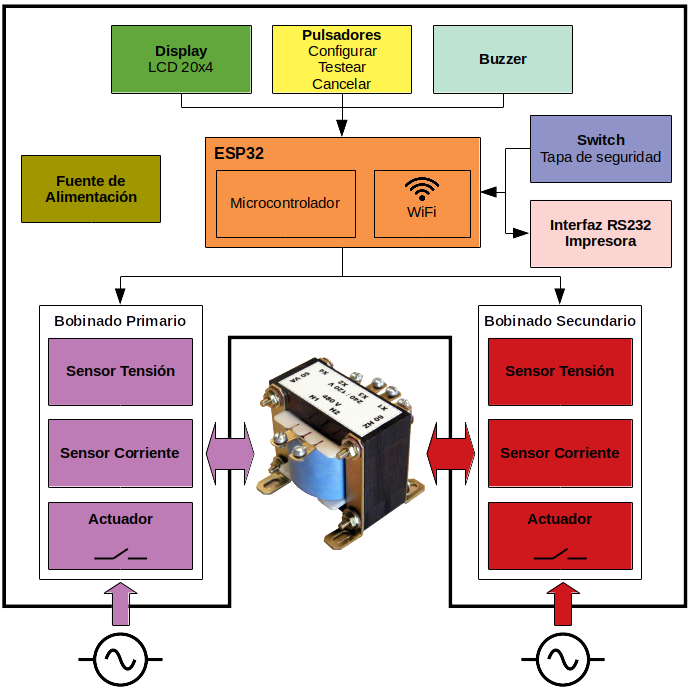
\includegraphics[width=.8\textwidth]{./Figures/diagBloques.png}
\caption{Diagrama en bloques del sistema.}
\label{fig:diagBloques}
\end{figure}


En la figura \ref{fig:FSMSimplificada} se presenta un diagrama de secuencia simplificado del dispositivo cuyos estados se describen a continuación:

\begin{figure}[htpb]
\centering 
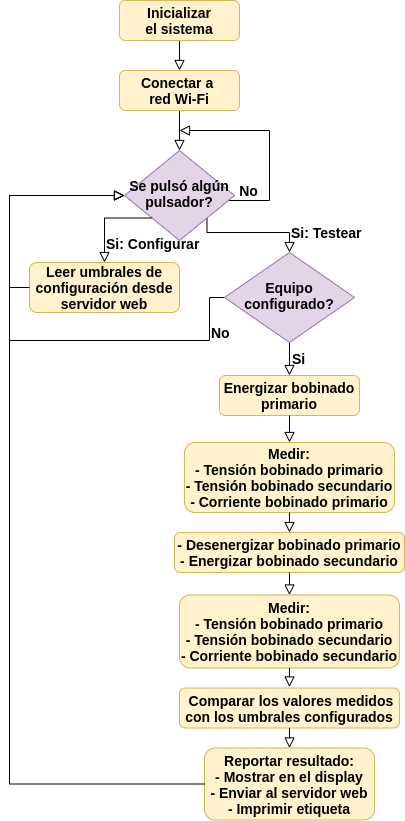
\includegraphics[width=.8\textwidth]{./Figures/FSMSimplificada.png}
\caption{Diagrama de secuencia simplificado.}
\label{fig:FSMSimplificada}
\end{figure}

\begin{enumerate}
\item Inicialización del sistema.
\item Conexión a red Wi-Fi.
\item Espera por pulsadores. El operador debe pulsar Configurar para leer los umbrales de configuración desde el servidor web.
\item Luego, el operador debe pulsar Testear para iniciar la caracterización del transformador. Aquí se verifica que el equipo haya sido configurado previamente ya que no se puede caracterizar un transformador si no cuenta con los umbrales de comparación. En caso de estar configurado se procede a los siguientes pasos.
\item Energizar el bobinado primario con 230 V$_{RMS}$ estabilizados (provistos externamente por el cliente).
\item Medir:
\begin{itemize}
	\item Tensión en bobinado primario.
	\item Corriente que circula por el bobinado primario.
	\item Tensión en bobinado secundario.
\end{itemize}
\item Desenergizar el bobinado primario.
\item Energizar el bobinado secundario con la tensión adecuada. Esta tensión se genera internamente a partir de la tensión de 230 V$_{RMS}$.
\item Medir:
\begin{itemize}
	\item Tensión en bobinado primario.
	\item Tensión en bobinado secundario.
	\item Corriente que circula por el bobinado secundario.
\end{itemize}
\item Desenergizar el bobinado secundario.
\item Comparar los valores medidos con los umbrales configurados previamente y determinar si el transformador es aceptado o rechazado.
\item Reportar los valores medidos y los resultados obtenidos al:
\begin{itemize}
	\item Servidor web.
	\item En el \textit{display} local.
	\item Imprimir una etiqueta.
\end{itemize}
\end{enumerate}


\section{Requerimientos}

A continuación se enumeran los requerimientos consensuados con el cliente:

\subsection{Requerimientos de hardware}
	\begin{enumerate}
	\item El dispositivo debe ser diseñado en base al módulo ESP32.
	\item El dispositivo debe ser capaz de medir tensiones y corrientes alternas de manera aislada del transformador bajo ensayo.
	\item El dispositivo debe ser capaz de conmutar las tensiones primarias y secundarias.
	\item El dispositivo debe tener un \textit{display} LCD alfanumérico de 20x4 caracteres.
	\item El dispositivo debe tener una interfaz Wi-Fi.
	\item El dispositivo debe tener una interfaz RS232 capaz de manejar impresoras series.
	\item El dispositivo debe alimentarse desde la red eléctrica Argentina 220 V$_{RMS}$/50 hz, debiendo proveerse todas las alimentaciones a los diferentes módulos de hardware.
	\item El dispositivo debe poseer un \textit{switch} para indicar que la tapa de seguridad ha sido removida.
	\item El dispositivo debe poseer tres pulsadores nombrados Configurar, Testear y Cancelar.
	\item El dispositivo debe poseer un \textit{buzzer}.
	\end{enumerate}
\subsection{Requerimientos relativos a los valores a medir}
	\begin{enumerate}
	\item Bobinado primario:
		\begin{enumerate}
		\item Rango tensión: 100 – 240 V$_{RMS}$.
		\item Rango corriente: 0 – 800 mA$_{RMS}$.
		\end{enumerate}
	\item Bobinado secundario:
		\begin{enumerate}
		\item Rango tensión: 0 – 30 V$_{RMS}$.
		\item Rango corriente: 0 – 1500 mA$_{RMS}$.
		\end{enumerate}
	\item Precisión en la medición de tensión: mejor al 1,5\% (puede variar en base a lo que se pueda conseguir en el mercado).
	\item Precisión en la medición de corriente: mejor al 4\% (puede variar en base a lo que se pueda conseguir en el mercado).
	\end{enumerate}
\subsection{Requerimientos funcionales}
	\begin{enumerate}
	\item El dispositivo debe permitir que se configuren los umbrales mínimos y máximos para los parámetros medidos. 
	\item Los valores a configurar deben ser adquiridos solo por Wi-Fi, no se admite configuración local por teclado.
	\item El dispositivo debe generar una confirmación de aceptación o rechazo del transformador en ensayo basado en los umbrales mínimos y máximos preseteados.
	\item El dispositivo, luego de cada ensayo, independientemente del resultado, debe imprimir una etiqueta con la siguiente información:
		\begin{enumerate}
		\item Número de partida del transformador ensayado.
		\item Condición de aceptado o rechazado.
		\item Valores medidos de tensiones y corrientes.
		\end{enumerate}
	\end{enumerate}	
\subsection{Requerimientos de comunicación}
	\begin{enumerate}
	\item Solicitar parámetros de configuración: el dispositivo debe generar un comando GET de HTTP a un servidor web (provisto por el cliente) para obtener los umbrales de aceptación y el número de partida del transformador a ensayar.
	\item El dispositivo debe ser capaz de procesar la respuesta del comando GET que está en formato JSON.
	\item Enviar resultados del ensayo: el dispositivo debe generar un comando POST de HTTP a un servidor (provisto por el cliente) con la información del transformador ensayado en formato JSON.
	\end{enumerate}
\subsection{Requerimientos de interfaz de usuario}
\label{subsec:ReqUsu}
	\begin{enumerate}
	\item Sobre la funcionalidad de los pulsadores:
		\begin{enumerate}
		\item Configurar: al pulsar este pulsador el dispositivo debe generar el comando GET para solicitar al servidor web los parámetros de configuración del dispositivo a través de Wi-Fi.
		\item Testear: al pulsar este pulsador el dispositivo debe iniciar la secuencia de testeo.
		\item Cancelar: al pulsar este pulsador la secuencia de testeo en curso debe quedar abortada.
		\end{enumerate}
	\item Sobre la funcionalidad del \textit{display} LCD:
		\begin{enumerate}
		\item El dispositivo debe mostrar los umbrales configurados y los valores de las mediciones actuales.
		\item Los valores de los umbrales configurados deberán permanecer en el \textit{display} durante el ensayo.
		\item El dispositivo debe mostrar los valores medidos del transformador ensayado luego de cada medición.
		\item Luego de finalizado el ensayo, se debe mostrar un mensaje que indique que la información se ha enviado al servidor web y mantenerse el dispositivo bloqueado hasta que se haya recibido la respuesta del servidor.
		\end{enumerate}
	\item Sobre el \textit{buzzer}:
		\begin{enumerate}
		\item El dispositivo debe emitir un solo sonido de 0,5 segundos de duración para confirmar la aceptación del transformador.
		\item El dispositivo debe emitir un sonido de repetición de 5 ciclos de 0,5 segundos de duración, con pausas de 0,5 segundos para confirmar el rechazo del transformador.
		\end{enumerate}		
	\end{enumerate}


\section{Kit ESP32-DevKitC}

Para este trabajo se utilizó el kit de desarrollo ESP32-DevKitC \citep{ESP32} desarrollado por la empresa Espressif Systems, figura \ref{fig:ESP32DevKitC}. Este kit integra un módulo ESP32-WROOM-32 \citep{WROOM} de la misma empresa, figura \ref{fig:ESP32WROOM}. El módulo ESP32-WROOM-32 es un microcontrolador de doble núcleo con interfaces Wi-Fi y Bluetooth. Además de las interfaces anteriores, el módulo cuenta con interfaces UART, SPI, numerosas entradas-salidas de propósito general, conversores analógico-digital y conversores digital-analógico.

\begin{figure}[htpb]
	\centering
	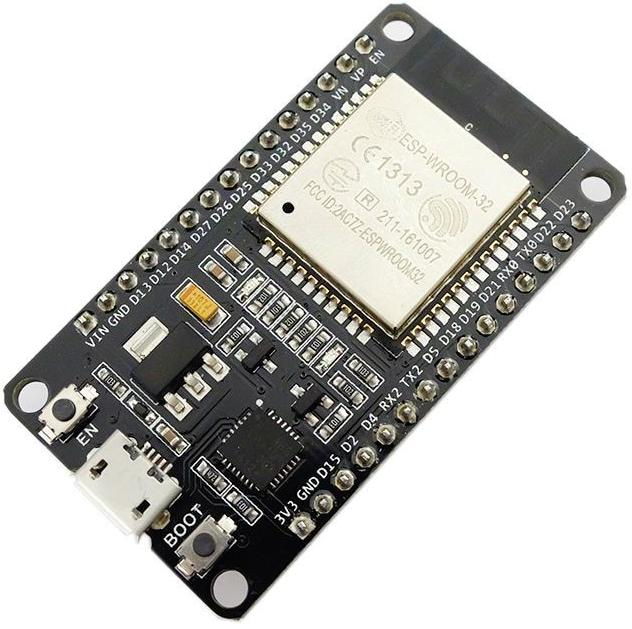
\includegraphics[scale=1.2]{./Figures/ESP32DevKit.jpg}
	\caption{ESP32-DevKitC V1.}
	\label{fig:ESP32DevKitC}
\end{figure}

\begin{figure}[htpb]
	\centering
	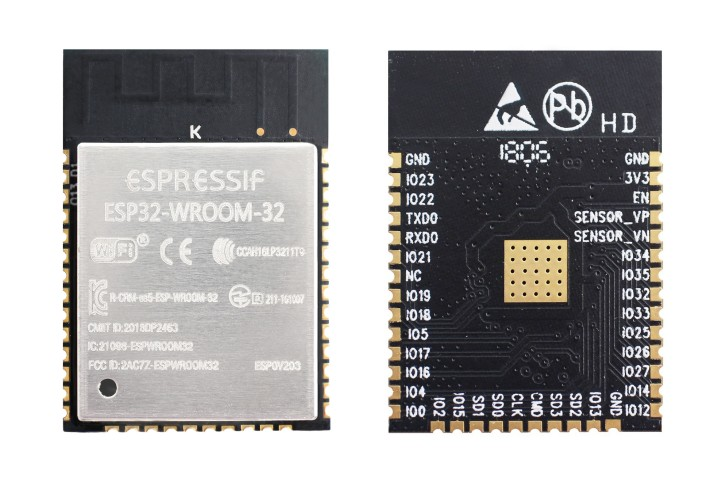
\includegraphics[scale=.5]{./Figures/esp32-wroom-32-front-back.jpg}
	\caption{ESP32-WROOM-32.}
	\label{fig:ESP32WROOM}
\end{figure}

De las especificaciones del módulo ESP32-WROOM-32 se pueden destacar las siguientes:
\begin{itemize}
\item Procesador dual core Xtensa® LX6 de 32 bits.
\item Velocidad de reloj de hasta 240 Mhz.
\item 520 KB de RAM.
\item 4 MB SPI flash.
\item Wi-Fi integrado con posibilidad de trabajar como AP (\textit{Access Point}) y SM (\textit{Station Mode}).
\item Bluetooth V4.2.
\item 36 GPIO.
\item Hasta 18 conversores anologico-digital (ADC) de 12 bits de resolución.
\item 2 conversores digital-analógico (DAC) de 8 bits de resolución.
\item 3 UART.
\item 2 canales I2C.
\item 4 canales SPI.
\item Interfaz JTAG.
\end{itemize}

Dado que el ESP32-DevKitC integra al módulo ESP32-WROOM-32, puede que no todos sus periféricos y entradas-salidas de propósito general (GPIO por sus siglas en inglés) estén disponibles. 

A continuación se detallan las principales características del kit ESP32-DevKitC:
\begin{itemize}
\item Doble hilera de pines con casi todas las entradas-salidas de propósito general del ESP32-WROOM-32.
\item Puente USB-UART conectado al módulo ESP32-WROOM-32. Esta interfaz es muy útil para programación y depuración.
\item Regulador LDO para proveer alimentación a los elementos del kit. 
\end{itemize}

\subsection{Entorno de desarrollo ESP-IDF}
\label{sec:ESPIDF}
%https://docs.espressif.com/projects/esp-idf/en/latest/esp32/about.html#:~:text=The\%20ESP\%2DIDF\%2C\%20Espressif\%20IoT,and\%20Mac\%20OS\%20operating\%20systems.

Espressif Systems provee un entorno de desarrollo de software denominado ESP-IDF \citep{ESPIDF}. El entorno ESP-IDF contiene todo lo necesario para desarrollar aplicaciones para los módulos ESP-32 sobre cualquier sistema operativo: Windows, Linux o MAC OS. Este entorno de desarrollo es \textit{Open-Source} y puede ser clonado desde un repositorio de GitHub\footnote{Repositorio GitHub para el ESP-IDF \url{https://docs.platformio.org/en/latest/frameworks/espidf.html}}. La empresa constantemente realiza actualizaciones y correcciones de fallas.

A continuación se listan algunas de las características más destacables del entorno ESP-IDF:

\begin{itemize}
\item Soporta \textit{FreeRTOS} \citep{ESPIDF:FreeRTOS}.
\item Soporta diferentes controladores de periféricos (SPI, I2C, UART, GPIO, I2S, ADC, DAC, etc) \citep{ESPIDF:PER}.
\item Soporta librerías para Wi-Fi \citep{ESPIDF:WiFi} y Bluetooth \citep{ESPIDF:bluetooth}.
\item Soporta varios \textit{stacks} de redes, por ejemplo TCP/IP.
\item Soporta varias implementaciones de protocolos (DHCP cliente y servidor, HTTP cliente y servidor, MQTT, etc) \citep{ESPIDF:PRO}.
\item Soporta extensiones para Eclipse \citep{ESPIDF:ECLIPSE} y Visual Code \citep{ESPIDF:VC}.
\item Está basado en CMake \citep{ESPIDF:CMake}.
\end{itemize}

El entorno ESP-IDF no es parte del proyecto del usuario sino que debe ser enlazado por medio de la variable de entorno IDF\_PATH. Esto último ayuda a separar el entorno de desarrollo del proyecto particular del usuario. Para utilizar ESP-IDF se requiere una estructura particular de archivos y carpetas para el proyecto \citep{ESPIDF:CMake_2}. 

\subsection{ESP-Touch y SmartConfig}
\label{sec:ESPTouch}

Espressif Systems provee la aplicación móvil ESP-Touch \citep{ESPTOUCH} la cual puede ser usada con la librería SmartConfig \citep{SMARTCONFIG} para configurar las credenciales de Wi-Fi en equipos que no posean una interfaz de usuario acorde para insertar esta información. En la figura \ref{fig:EspTouch} se muestra la interfaz de la aplicación ESP-Touch.

\begin{figure}[htpb]
	\centering
	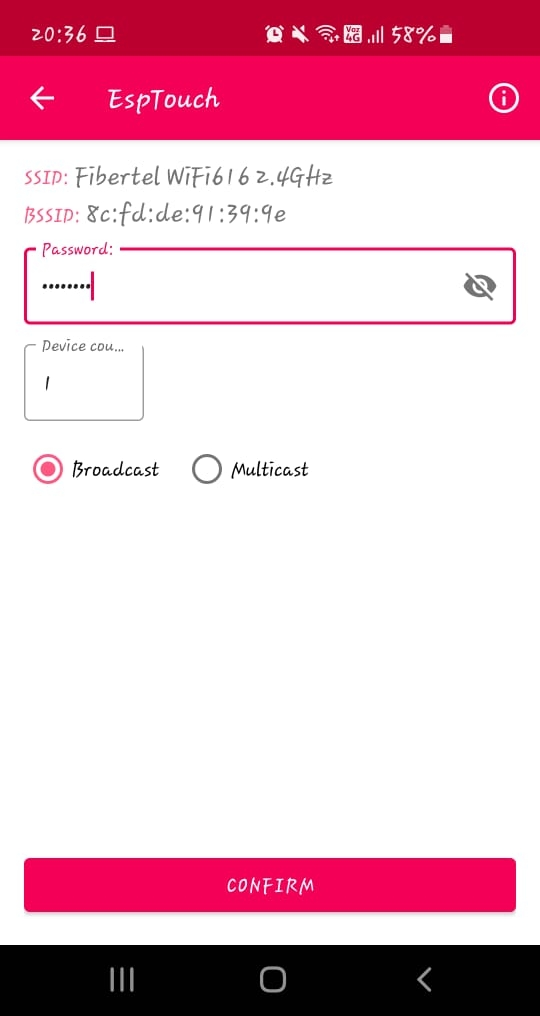
\includegraphics[scale=.5]{./Figures/EspTouch.jpeg}
	\caption{Aplicación Android ESP-Touch.}
	\label{fig:EspTouch}
\end{figure}

La ventaja de esta tecnología es que el dispositivo no necesita conocer directamente el SSID o la contraseña de un punto de acceso (AP), en cambio esta información se proporciona mediante el teléfono móvil. ESP-Touch está disponible para Android e iOS.

\section{Sensor de tensión}
\label{sec:secZMPT101B}

Para monitorear las tensiones del bobinado primario y secundario se utilizó el módulo de figura \ref{fig:ZMPT101B}.

\begin{figure}[htpb]
	\centering
	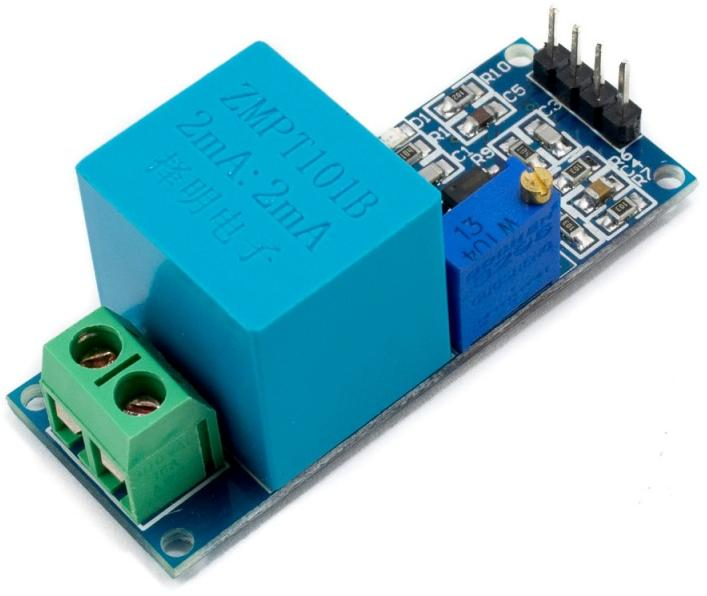
\includegraphics[scale=.3]{./Figures/zmpt101b.jpg}
	\caption{Módulo sensor de tensión alterna.}
	\label{fig:ZMPT101B}
\end{figure}

Este módulo es un sensor de tensión capaz de medir tensiones alternas de línea de 220 V$_{RMS}$ de forma aislada. En la figura \ref{fig:ZMPT101B_waves} se puede observar la tensión de entrada (Vin) y la tensión de salida (Vout) entregada por el módulo. El módulo provee una tensión de salida la cual está montada sobre un nivel continua igual a la mitad de la tensión de alimentación, esto ayuda a procesar la señal directamente con un ADC sin la necesidad de fuentes de alimentación negativas.

\begin{figure}[htpb]
	\centering
	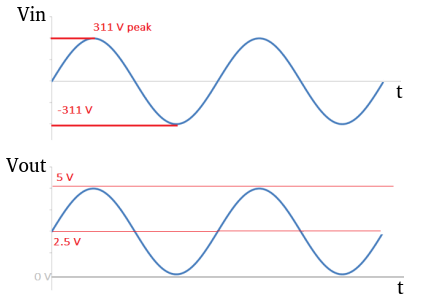
\includegraphics[scale=1.2]{./Figures/ZMPT101B_waves.png}
	\caption{Ondas de entrada (Vin) y salida (Vout) del módulo @ Vcc = 5 V.}
	\label{fig:ZMPT101B_waves}
\end{figure}

El elemento principal del módulo es el transformador de corriente ZMPT101B de la empresa Qingxian Zeming Langxi Electronic \citep{ZMPT101B_b}. Este componente es el encargado de proporcionar la aislación entre la alta tensión de línea y la baja tensión hacia el microcontrolador. El primario del transformador se conecta a la tensión alterna de la red a través de la bornera verde que se observa en la figura \ref{fig:ZMPT101B}. En el lado secundario del transformador se tiene una resistencia serie (\textit{shunt}) y un circuito amplificador basado en el operacional LM358 \citep{LM358}. Adicionalmente, el circuito posee un potenciómetro para ajustar la ganancia del sistema.

Este módulo se utiliza en aplicaciones de domótica e IoT (Internet of Things) para el monitoreo de la tensión de línea.

Especificaciones técnicas del módulo: 
\begin{itemize}
\item Tensión de alimentación (Vcc): 5-30 V.
\item Tensión alterna de entrada máxima: 250 V$_{RMS}$.
\item Tensión de salida: onda senoidal 2,5 V$_{PICO}$ @ Vcc = 5 V.
\item Valor medio de la tensión salida: 2,5 V @ Vcc = 5 V.
\item Dimensiones: 5 cm x 2 cm x 2,4 cm.
\end{itemize}

\section{Sensor de corriente}
\label{sec:secZMCT103C}

Para monitorear las corrientes del bobinado primario y secundario se utilizó el módulo de figura \ref{fig:ZMCT103C}.

\begin{figure}[htpb]
	\centering
	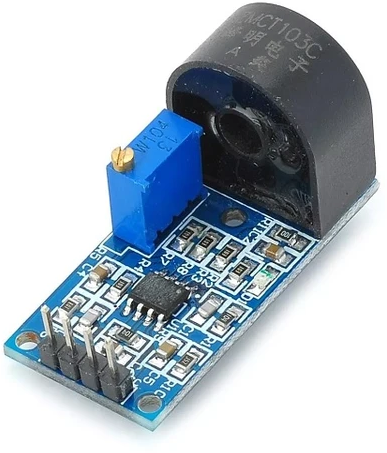
\includegraphics[scale=.5]{./Figures/ZMCT103C.png}
	\caption{Módulo sensor de corriente alterna.}
	\label{fig:ZMCT103C}
\end{figure}

Este módulo facilita el monitoreo de corriente alternas de hasta 5 A$_{RMS}$. Está basado en el transformador de corriente de alta precisión ZMCT103C de la empresa Qingxian Zeming Langxi Electronic \citep{ZMCT103C_b}. El módulo es similar al módulo sensor de tensión presentado en la sección \ref{sec:secZMPT101B}. La corriente de salida del transformador de corriente pasa por una resistencia serie (\textit{shunt}) y luego es acondicionada por los amplificadores operaciones integrados en el LM358 \citep{LM358}. La única diferencia entre el módulo sensor de corriente y el de tensión, es que el primero entrega una tensión alterna con valor medio cero, es decir, sin componente de continua. Esto último hace necesario alguna modificación adicional del módulo para entregar una tensión que sea siempre positiva.

Especificaciones técnicas del módulo: 
\begin{itemize}
\item Tensión de alimentación (Vcc): 5-30 V.
\item Corriente de entrada nominal: 5 A$_{RMS}$.
\item Tensión de salida: onda senoidal 2.5 V$_{PICO}$ @ Vcc = 5 V.
\item Valor medio de la tensión salida: 0 V @ Vcc = 5 V.
\end{itemize}

\section{Impresora}
\label{sec:Impre}
Para este trabajo se utilizó una impresora de transferencia térmica modelo E-Class™ Mark III fabricada por Honeywell \citep{printer_b}, ver figura \ref{fig:printer}. Las impresoras por transferencia térmica utilizan una cinta de tinta denominada \textit{Ribbon} que con el calor del cabezal derrite la tinta sobre el papel. Este fenómeno permite imprimir códigos de barras, textos, etc. Estas impresoras son de bajo costo pero ofrecen como desventaja que solo imprimen en blanco y negro.

\begin{figure}[htpb]
	\centering
	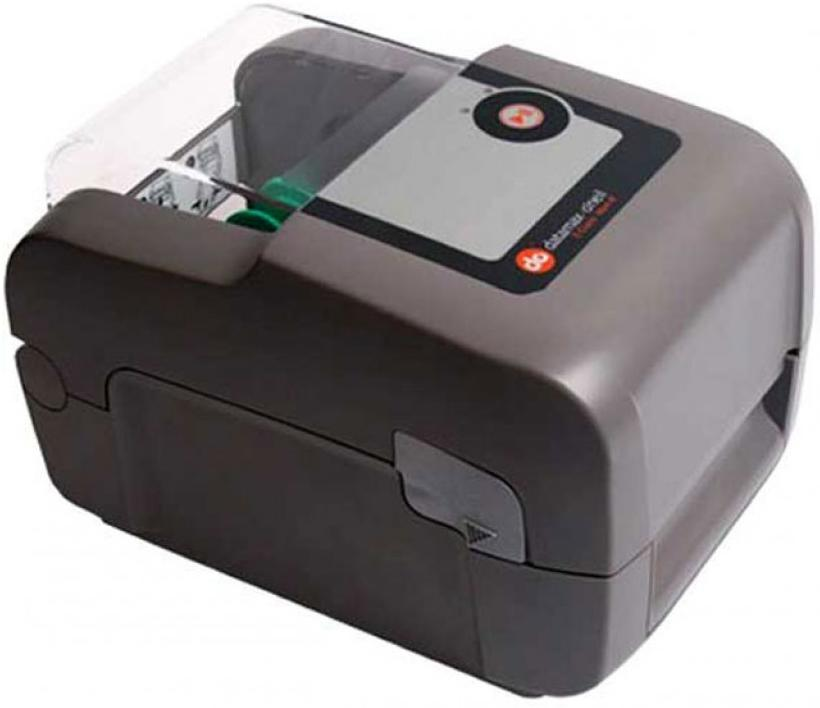
\includegraphics[scale=0.3]{./Figures/printer.jpeg}
	\caption{Impresora E-Class™ Mark III modelo E-4204B.}
	\label{fig:printer}
\end{figure}


Especificaciones técnicas del modelo E-4204B:
\begin{itemize}
\item Resolución: 8 puntos/mm (203 ppp).
\item Velocidad máxima de impresión: 101 mm/s (4 pps).
\item Ancho máximo de papel: 112 mm.
\item Capacidad de rollo: diámetro externo 127 mm.
\item Memoria: DRAM de 16 MB/Flash de 8 MB.
\item Comunicación: USB 2.0 y RS232 serie.
\item Lenguajes soportados: DPL(Datamax), ZPL(Zebra), EPL(Eltron), BPL(Boca), IPL(Intermec).
\item Indicadores de estado: dos indicadores luminosos de tres colores.
\item Dimensiones: 187 mm x 203,5 mm x 282 mm.
\item Peso: 2,4 Kg.
\end{itemize}

\subsection{Protocolo DPL}
\label{subsec:ProDPL}
El protocolo DPL (Datamax-O’Neil \textit{Programming Language}) es un protocolo propietario de la firma Datamax el cual puede ser utilizado para comunicarse con las impresoras E-Class™ Mark III \citep{DPL_man}. Este es un protocolo punto a punto de tipo ASCII basado en la arquitectura maestro/esclavo. La impresora se conecta con el \textit{host} sin intermediarios.

El protocolo está formado por comandos y parámetros asociados a estos comandos. En la tabla \ref{tab:printercmd} se muestran los comandos disponibles.

\begin{table}[htpb]
\centering
\caption[Comandos protocolo DPL]{Tipos de comandos protocolo DPL.}
\resizebox{\textwidth}{!}{%
\begin{tabular}{c c c}
\hline
\toprule
\textbf{ASCII (HEX)} & \textbf{Tipo}     & \textbf{Descripción}\\
\midrule
SOH (0x01)  & Comando inmediato          & \begin{tabular}[c]{@{}c@{}}Cuando la impresora recibe un comando inmediato, \\interrumpe su operación actual y pasa a ejecutarlo. \\Ejemplos: reinicio de la impresora, \\pedido de estado de la impresora.\end{tabular}                         \\ \hline
STX (0x02)  & Comando de sistema          & \begin{tabular}[c]{@{}c@{}}Es el tipo de comando más comúnmente utilizado. \\Ejemplos: configurar el modo de trabajo métrico o \\imperial, tipo de alineación del texto a imprimir, indica el \\inicio y fin del texto a imprimir, etc.\end{tabular} \\ \hline
ESC (0x1B)  & \begin{tabular}[c]{@{}c@{}}Comando de carga de\\fuente \end{tabular}& \begin{tabular}[c]{@{}c@{}}Este comando es utilizado para cargar una nueva fuente. \\Generalmente es utilizado por programas\\ específicos para la creación de fuentes.\end{tabular}\\ 
\bottomrule
\hline
\end{tabular}%
}
\label{tab:printercmd}
\end{table}

En las siguientes secciones se describen los comandos inmediatos y los comandos de sistema ya que fueron los utilizados en este trabajo.

\subsubsection{Comandos inmediatos}
\label{subsubsec:ProDPLCMDIn}
En la tabla \ref{tab:printercmdInmediatos} se muestran los comandos inmediatos más utilizados, en la última columna se muestra la respuesta de la impresora.

\begin{table}[htpb]
\centering
\caption[Comandos inmediatos protocolo DPL]{Comandos inmediatos protocolo DPL.}
\resizebox{\textwidth}{!}{%
\begin{tabular}{c c l}
\toprule
\textbf{ASCII (HEX)} & \textbf{Descripción} & \multicolumn{1}{c}{\textbf{Respuesta}}\\ 
\midrule
\begin{tabular}[c]{@{}c@{}}\textless{}SOH\textgreater{}A\textless{}CR\textgreater\\ (0x01,0x41,0x0D)\end{tabular} & \begin{tabular}[c]{@{}c@{}}Pedido de estado de la impresora.\end{tabular} & \begin{tabular}[c]{@{}l@{}}La respuesta son 8 caracteres 'Y' o 'N' \\mas el carácter \textless{}CR\textgreater{} de final de mensaje.\\ \\ abcdefgh\textless{}CR\textgreater\\ a: Interprete de comandos ocupado\\ b: Falla de papel\\ c: Falla del \textit{Ribbon}\\ d: Imprimiendo lote (se pueden enviar \\varias etiquetas para imprimir)\\ e: Impresora ocupada\\ f: Impresora pausada\\ g: Etiqueta presentada\\ h: Falla interna\end{tabular} \\
\begin{tabular}[c]{@{}c@{}}\textless{}SOH\textgreater{}*\textless{}CR\textgreater\\ (0x01,0x2A,0x0D)\end{tabular} & Pedido de reinicio de la impresora                                                                                                                                       & \textless{}XON\textgreater{}R\textless{}CR\textgreater{} \\ 
\bottomrule
\hline
\end{tabular}%
}
\label{tab:printercmdInmediatos}
\end{table}

En el caso del comando \textless{}SOH\textgreater{}A\textless{}CR\textgreater{}, la respuesta de la impresora es una cadena del tipo ``YYNYYNYY\textless{}CR\textgreater{}'', donde cada carácter 'Y' o 'N' se corresponde con los caracteres ``abcdefgh\textless{}CR\textgreater{}'' de la tabla \ref{tab:printercmdInmediatos}. Para poder imprimir, la impresora debe devolver la cadena ``YYYYYYYY\textless{}CR\textgreater{}'' la cual indica que no tiene errores ni está ocupada con otra tarea.

\subsubsection{Comandos de sistema}

El principal uso de los comandos de sistema es enviar a la impresora los caracteres que se desean imprimir. Además de los caracteres a imprimir, se pueden configurar diferentes aspectos de la impresora tales como: temperatura del cabezal, alineación del texto, tipo y tamaño de la fuente, posición del texto, etc.

El comando \textless{}STX\textgreater{}L\textless{}CR\textgreater{} es el más utilizado. Este comando permite enviarle a la impresora una línea de texto a imprimir con su formato y ubicación. En la tabla \ref{tab:printercmdSystem} se muestra el formato para imprimir una línea de texto. % Pag 163

\begin{table}[htpb]
\centering
\caption[Comandos de sistema protocolo DPL]{Comandos de sistema protocolo DPL.}
\resizebox{\textwidth}{!}{%
\begin{tabular}{c c c c c}
\hline
\toprule
\textbf{Mensaje} & \textbf{Tipo} & \textbf{Descripción} & \begin{tabular}[c]{@{}c@{}}\textbf{Cantidad de} \\ \textbf{caracteres}\end{tabular} & \textbf{Ejemplo} \\ 
\midrule
a      & Número     & \begin{tabular}[c]{@{}c@{}}Dirección de rotación del texto:\\ 1 = 0º, 2 = 90º, 3 = 180º, 4 = 270º\end{tabular} & 1 & 1 \\
b      & Número     & Fuente a utilizar                                                                                              & 1 & 3 \\
c      & Número     & Multiplicador de ancho de fuente                                                                               & 1 & 1 \\
d      & Número     & Multiplicador de alto de fuente                                                                                & 1 & 1 \\
eee    & Número     & 000                                                                                                            & 3 & 000 \\
ffff   & Número     & Posición vertical del texto en mm                                                                              & 4 & 0140 \\
gggg   & Número     & Posición horizontal del texto en mm                                                                            & 4 & 0000 \\
jj...j & Caracteres & Texto a imprimir                                                                                              & \begin{tabular}[c]{@{}c@{}}Largo de \\la cadena\end{tabular} & 10K OHM 1/4 WATT \\ 
\bottomrule
\hline
\end{tabular}%
}
\label{tab:printercmdSystem}
\end{table}

En el ejemplo de la tabla \ref{tab:printercmdSystem} se imprime la etiqueta mostrada en le figura \ref{fig:label_ej}.

\begin{figure}[htpb]
	\centering
	
\includegraphics[scale=0.3]{./Figures/label_ej.png}
	\caption{Etiqueta resultante del comando de la columna Ejemplo de la tabla \ref{tab:printercmdSystem}.}
	\label{fig:label_ej}
\end{figure}

Se pueden enviar varias líneas a imprimir en un solo comando, en este caso, para indicar el fin del texto se debe enviar E\textless{}CR\textgreater.

\subsection{Módulo adaptador RS232}
\label{subsec:Mod232}
Para comunicar la impresora con la UART del microcontrolador se utilizó el módulo de la figura \ref{fig:rs232}. 

\begin{figure}[hb]
	\centering
	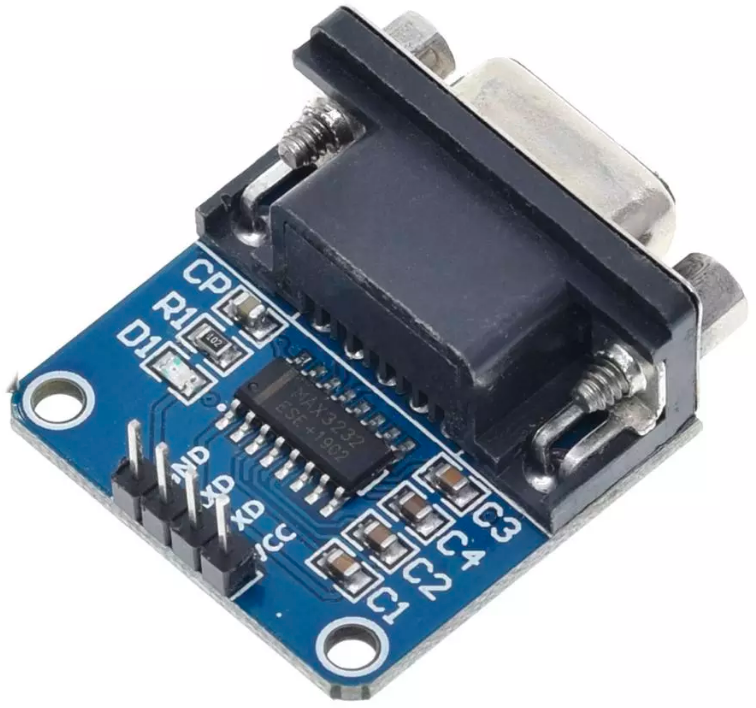
\includegraphics[scale=0.25]{./Figures/rs3232.png}
	\caption{Módulo adaptador RS232 a TTL.}
	\label{fig:rs232}
\end{figure}

Este módulo está basado en el integrado MAX3232 \citep{MAX3232} y adapta las señales del capa física RS232 a valores acordes para trabajar con el microcontrolador.

\section{Display alfanumérico}

Para este trabajo se utilizó un \textit{display} alfanumérico de 20 columnas por 4 líneas con controlador HD44780 de Hitachi \citep{HD44780}, ver figura \ref{fig:display}.

\begin{figure}[htpb]
	\centering
	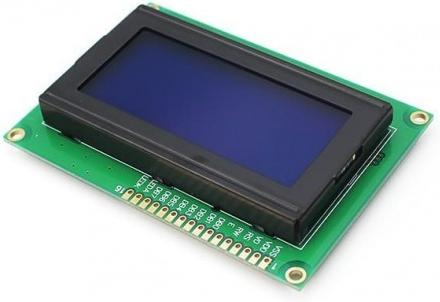
\includegraphics[scale=0.7]{./Figures/display.jpg}
	\caption{\textit{Display} alfanumérico de 20x4.}
	\label{fig:display}
\end{figure}

El display cuenta con una interfaz paralela de 8-bits (DB0-7) la cual puede ser utilizada en formato 4-bits haciendo 2 escrituras o lecturas. Cuenta también con tres líneas de control denominadas RS, R/W y EN. En la tabla \ref{tab:display} se muestran las señales necesarias para el manejo del \textit{display}.

\begin{table}[ht]
\centering
\caption[Señales de control y datos \textit{display}]{Señales de control y datos \textit{display}.}
\begin{tabular}{c c c}
\hline
\toprule
\textbf{Señal} & \begin{tabular}[c]{@{}c@{}}\textbf{Tamaño}\\ \textbf{bits}\end{tabular} & \textbf{Descripción} \\ 
\midrule
RS    & 1 & \begin{tabular}[c]{@{}c@{}}Indica como interpretar los datos en el \textit{bus} de datos DB.\\ 0: Instrucción\\ 1: Datos\end{tabular} \\
R/W   & 1 & \begin{tabular}[c]{@{}c@{}}0: Operación de lectura\\ 1: Operación de escritura\end{tabular} \\
EN    & 1 & \begin{tabular}[c]{@{}c@{}}\textit{Enable}: utilizado para indicar que hay \\ datos validos en el \textit{bus} de datos\end{tabular} \\
DB    & 8 & \textit{Bus} de datos \\
\bottomrule
\hline
\end{tabular}%
\label{tab:display}
\end{table}

Para utilizar el display se cuenta con 2 tipos de operaciones las cuales se diferencian por el bit de control RS:
\begin{itemize}
\item RS=0: Escribir/leer una instrucción.
\item RS=1: Escribir/leer un carácter ASCII.
\end{itemize}

\pagebreak

En la tabla \ref{tab:displayCmd} se muestran las instrucciones más utilizadas.

\begin{table}[htpb]
\centering
\caption[Instrucciones controlador HD44780]{Instrucciones más utilizadas para el controlador HD44780.}
\begin{tabular}{c c l}
\hline
\toprule
\textbf{Nombre} & \begin{tabular}[l]{@{}c@{}}\textbf{Valor}\\ \textbf{hexa}\end{tabular} & \textbf{Acción} \\ 
\midrule
Borrado         & 0x01 &  Borra la pantalla completa\\
Modo de entrada & 0x04 & \begin{tabular}[l]{@{}l@{}}Fijar dirección del cursor: izquierda o derecha\end{tabular} \\
\begin{tabular}[c]{@{}c@{}}Control de \\encendido y apagado\end{tabular} & 0x08 & \begin{tabular}[l]{@{}l@{}}- Encender o apagar la pantalla\\- Encender o apagar el cursor \end{tabular} \\
Fijar \textit{Set}    & 0x10 & \begin{tabular}[l]{@{}l@{}}- Fijar tamaño del \textit{bus} de datos \\- Fijar número de líneas \\- Fijar fuente de los caracteres \end{tabular} \\
\bottomrule
\hline
\end{tabular}%
\label{tab:displayCmd}
\end{table}

\section{Módulos misceláneos}

En esta sección se describe el módulo utilizado como elemento de maniobra para alimentar los bobinados del transformador y la fuente de alimentación utilizada en el trabajo.

\subsubsection{Módulo de relés}
\label{subsubsec:ModRel}

Para poder conmutar las tensiones aplicadas a los bobinados del transformador bajo ensayo se utilizó el módulo de la figura \ref{fig:reles} . Este módulo está compuesto por 8 relés los cuales pueden ser manejados en forma aislada por el microcontrolador a través de optoacopladores. Este módulo permitió actuar sobre las altas tensiones del transformador bajo ensayo de una manera segura.

\begin{figure}[htpb]
	\centering
	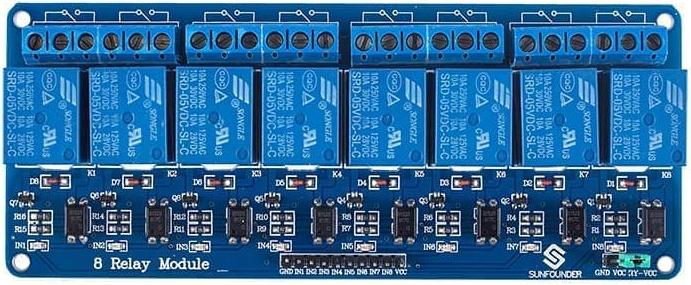
\includegraphics[scale=0.7]{./Figures/reles.jpeg}
	\caption{Módulo de relés.}
	\label{fig:reles}
\end{figure}

\pagebreak

\subsubsection{Módulo de alimentación}
\label{subsubsec:ModAlim}

El dispositivo diseñado debe ser alimentado desde la red eléctrica de Argentina (220 V$_{RMS}$ - 50 hz) para tal fin, se utilizó la fuente conmutada mostrada en la figura \ref{fig:fte}.

\begin{figure}[htpb]
	\centering
	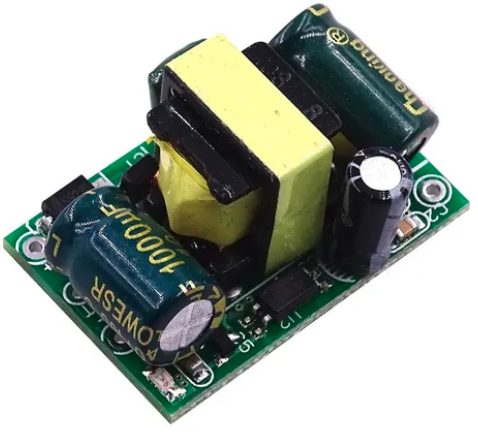
\includegraphics[scale=0.6]{./Figures/fte.png}
	\caption{Módulo de alimentación.}
	\label{fig:fte}
\end{figure}

Especificaciones técnicas\footnote{\url{https://articulo.mercadolibre.com.ar/MLA-700576819-fuente-aislada-switching-220v-5v-700ma-35w-20off-nut-_JM\#reco_item_pos=2&reco_backend=machinalis-v2p-pdp-boost-v2&reco_backend_type=low_level&reco_client=vip-v2p&reco_id=90222827-7627-46cb-9f2b-78620eec7ea2}}:
\begin{itemize}
\item Tensión de entrada: 85 a 265 V$_{RMS}$ 50 hz.
\item Corriente de entrada: 0,0273 A (110 V$_{RMS}$) y 0,014 A (220 V$_{RMS}$).
\item Tensión de salida: 5 V +/- 0,2 V.
\item Corriente de salida: 700 mA (800 mA$_{PICO}$).
\item Ripple: 60 mV.
\item Potencia: 3,5 W.
\item Eficiencia: 80\%.
\item Protección contra corto circuito.
\item Temperatura de operación: -20 a 60 $^{\circ}$C.
\end{itemize}



